\documentclass{csse4400}

% \teachermodetrue

\usepackage{float}

\usepackage{languages}

\title{Scaling Stateless Components}
\author{Evan Hughes \& Anna Truffet \& Brae Webb }

\date{\week[practical]{6}}
\begin{document}

\maketitle

\begin{figure}[h]
    \begin{center}
        
\includegraphics[scale=0.4]{images/scaling-out}
    \end{center}
\end{figure}

\section{This Week}
Our goal is to scale out the stateless component of our TaskOverflow application across multiple compute instances.
Specifically we will need to:
\begin{itemize}
    \item Route traffic to our deployed TaskOverflow application with a load balancer.
    \item Scale out TaskOverflow instances with autoscaling.
    \item Check the status of our instances with a healthcheck.
    \item Dynamically scale our application based on load.
\end{itemize}

\section{Load Balancers}

Load balancing distributes a load over a set of resources.
For example, balacing network traffic across several servers.
Load balancing is crucial to the scalability of modern systems, as often, one physical device can not process the large amount network traffic for (e.g.) a large website.

A service which load balances, is called a \textbf{Load Balancer}.


\subsection{Routing Algorithms}

A load balancer can implement many techinques to select which resource to route incoming requests toward, these techniques are the load balancer's routing algorithm.

Below lists several common routing techniques.
There are many other generic and bespoke routing algorithms that are not listed.

\begin{description}
  \item[Round Robin] allocates requests to the next available server regardless of where the last request was sent.
      It is simple, and in practice, works effectively.
  \item[Least Connections] sends the next request to the node with the fewest current connections.
      The load balancer is responsible for tracking how many connections exist to each node.
  \item[Weighted Least Connections] sends the next request to the node with the least weighted connections. This is similar to the above least connections method, however, each node has an associated weight.
      This allows certain nodes to be preferred over others.
      This is useful if we have an inequal distribution of compute power.
      We would want to give smaller nodes a reduced load in comparison to other more powerful nodes.
  \item[Consistent Hashing] In some cases we may want a user to consistently be routed to a specific node.
      This is useful for multiple transactions that need to be done in a consistent order or if the data is stored/cached on the node.
      This can be done by hashing the information in the request payload or headers and then routing the request to the node that handles hashes in the range of the computed hash.
\end{description}

\subsection{Health Checks}

When load balancing, it is important to ensure that the nodes we route requests to are able to service the request.
A good health check can save or break your service.
Consider the two following examples from UQ's Information Technology Services (ITS):

\paragraph{Example 1} Early in my career, I, Evan Hughes, setup a multi-node Directory Server at UQ under the hostname of \texttt{ldap.uq.edu.au}.
This server was a NoSQL database which implemented the LDAP protocol and supported \texttt{UQ Authenticate},
UQ's Single Sign-On service.

The service had a load balancer which checked that \texttt{port 389} is open and reachable. 
This worked well most of the time.
However, the health check was too weak. When:
\begin{enumerate} 
    \item A data-center outage occured; and
    \item The operating system running the service disappeared; but 
    \item The service was still running in memory.
\end{enumerate}

The health check passed, but in reality, the service was talking to dead nodes, causing upstream services to have intermitent failures. 

\todo{C4 Diagram of the architecture}

\paragraph{Example 2} During the rollout of a new prompt for UQ Authenticate which required users to go to my.UQ to provide verified contact details - the Blackboard (learn.uq.edu.au) service went completly offline.
The health check for Blackboard at the time completed a full authentication as a test user to ensure everything was functioning as expected.
Once this user was enrolled into the new rollout,
the health checks started reporting failures and within a matter of minutes the entire pool of nodes were shutdown.
This health check was too broad and was not isolated enough to the service that it was checking.

\todo{C4 diagram of the architecture}

A lot of services will provide a health check endpoint or a metrics endpoint which can help the engineer setup a proper level of health check.
We want a health check that is specific enough for the service that it is checking but not so specific that it is too brittle.
For the TaskOverflow application that we have been building so far,
a reasonable health check would be that the health endpoint ensures the database is available and that the application is able to connect to it.

\section{Load Balancers in AWS}

\subsection{Types of AWS Load Balancers}
Not all load balancers are the same.
Some load balancers inspect the transmitted packets to correctly route the packet.
We will cover two load balancer types AWS provides:

\begin{description}
  \item[Application Load Balancer] is an OSI layer 7%
\footnote{OSI layer 7: Application, in this case HTTP/HTTPS/etc}
load balancer which routes traffic based on the request's content.
      This is useful for services using HTTP, HTTPS, or any other supported protocol.
  \item[Network Load Balancer] is an OSI layer 4%
\footnote{OSI layer 4: Transport, in this case TCP/UDP}
load balancer which routes traffic based on the source and destination IP addresses and ports.
This is useful for services that are using TCP or UDP.
\end{description}

\subsection{AWS Load Balancer Design}

An AWS Elastic Load Balancer has three distinct components. 

\begin{description}
  \item[Listeners] allows traffic to enter the Elastic Load Balancer.
  Each listener has a port (e.g. \texttt{port 80}) and a protocol (e.g. \texttt{HTTP}) associated with it.
  \item[Target Groups] are groups of nodes which the load balancer can route to. 
      Each target group has a protocol and a port associated with it, allowing us (the programmer) to switch ports on the way through the load balancer.
      This is useful if the targets are using a different port to the ports we want to expose.
  \item[Load Balancer] is the actual load balancer that routes the traffic to the target groups based on rules that we setup.
      The load balancer has a DNS name that we can use to route traffic to it.
      The load balancer also has a security group that we can use to control what traffic can enter the load balancer. 
\end{description}

\begin{figure}[H]
  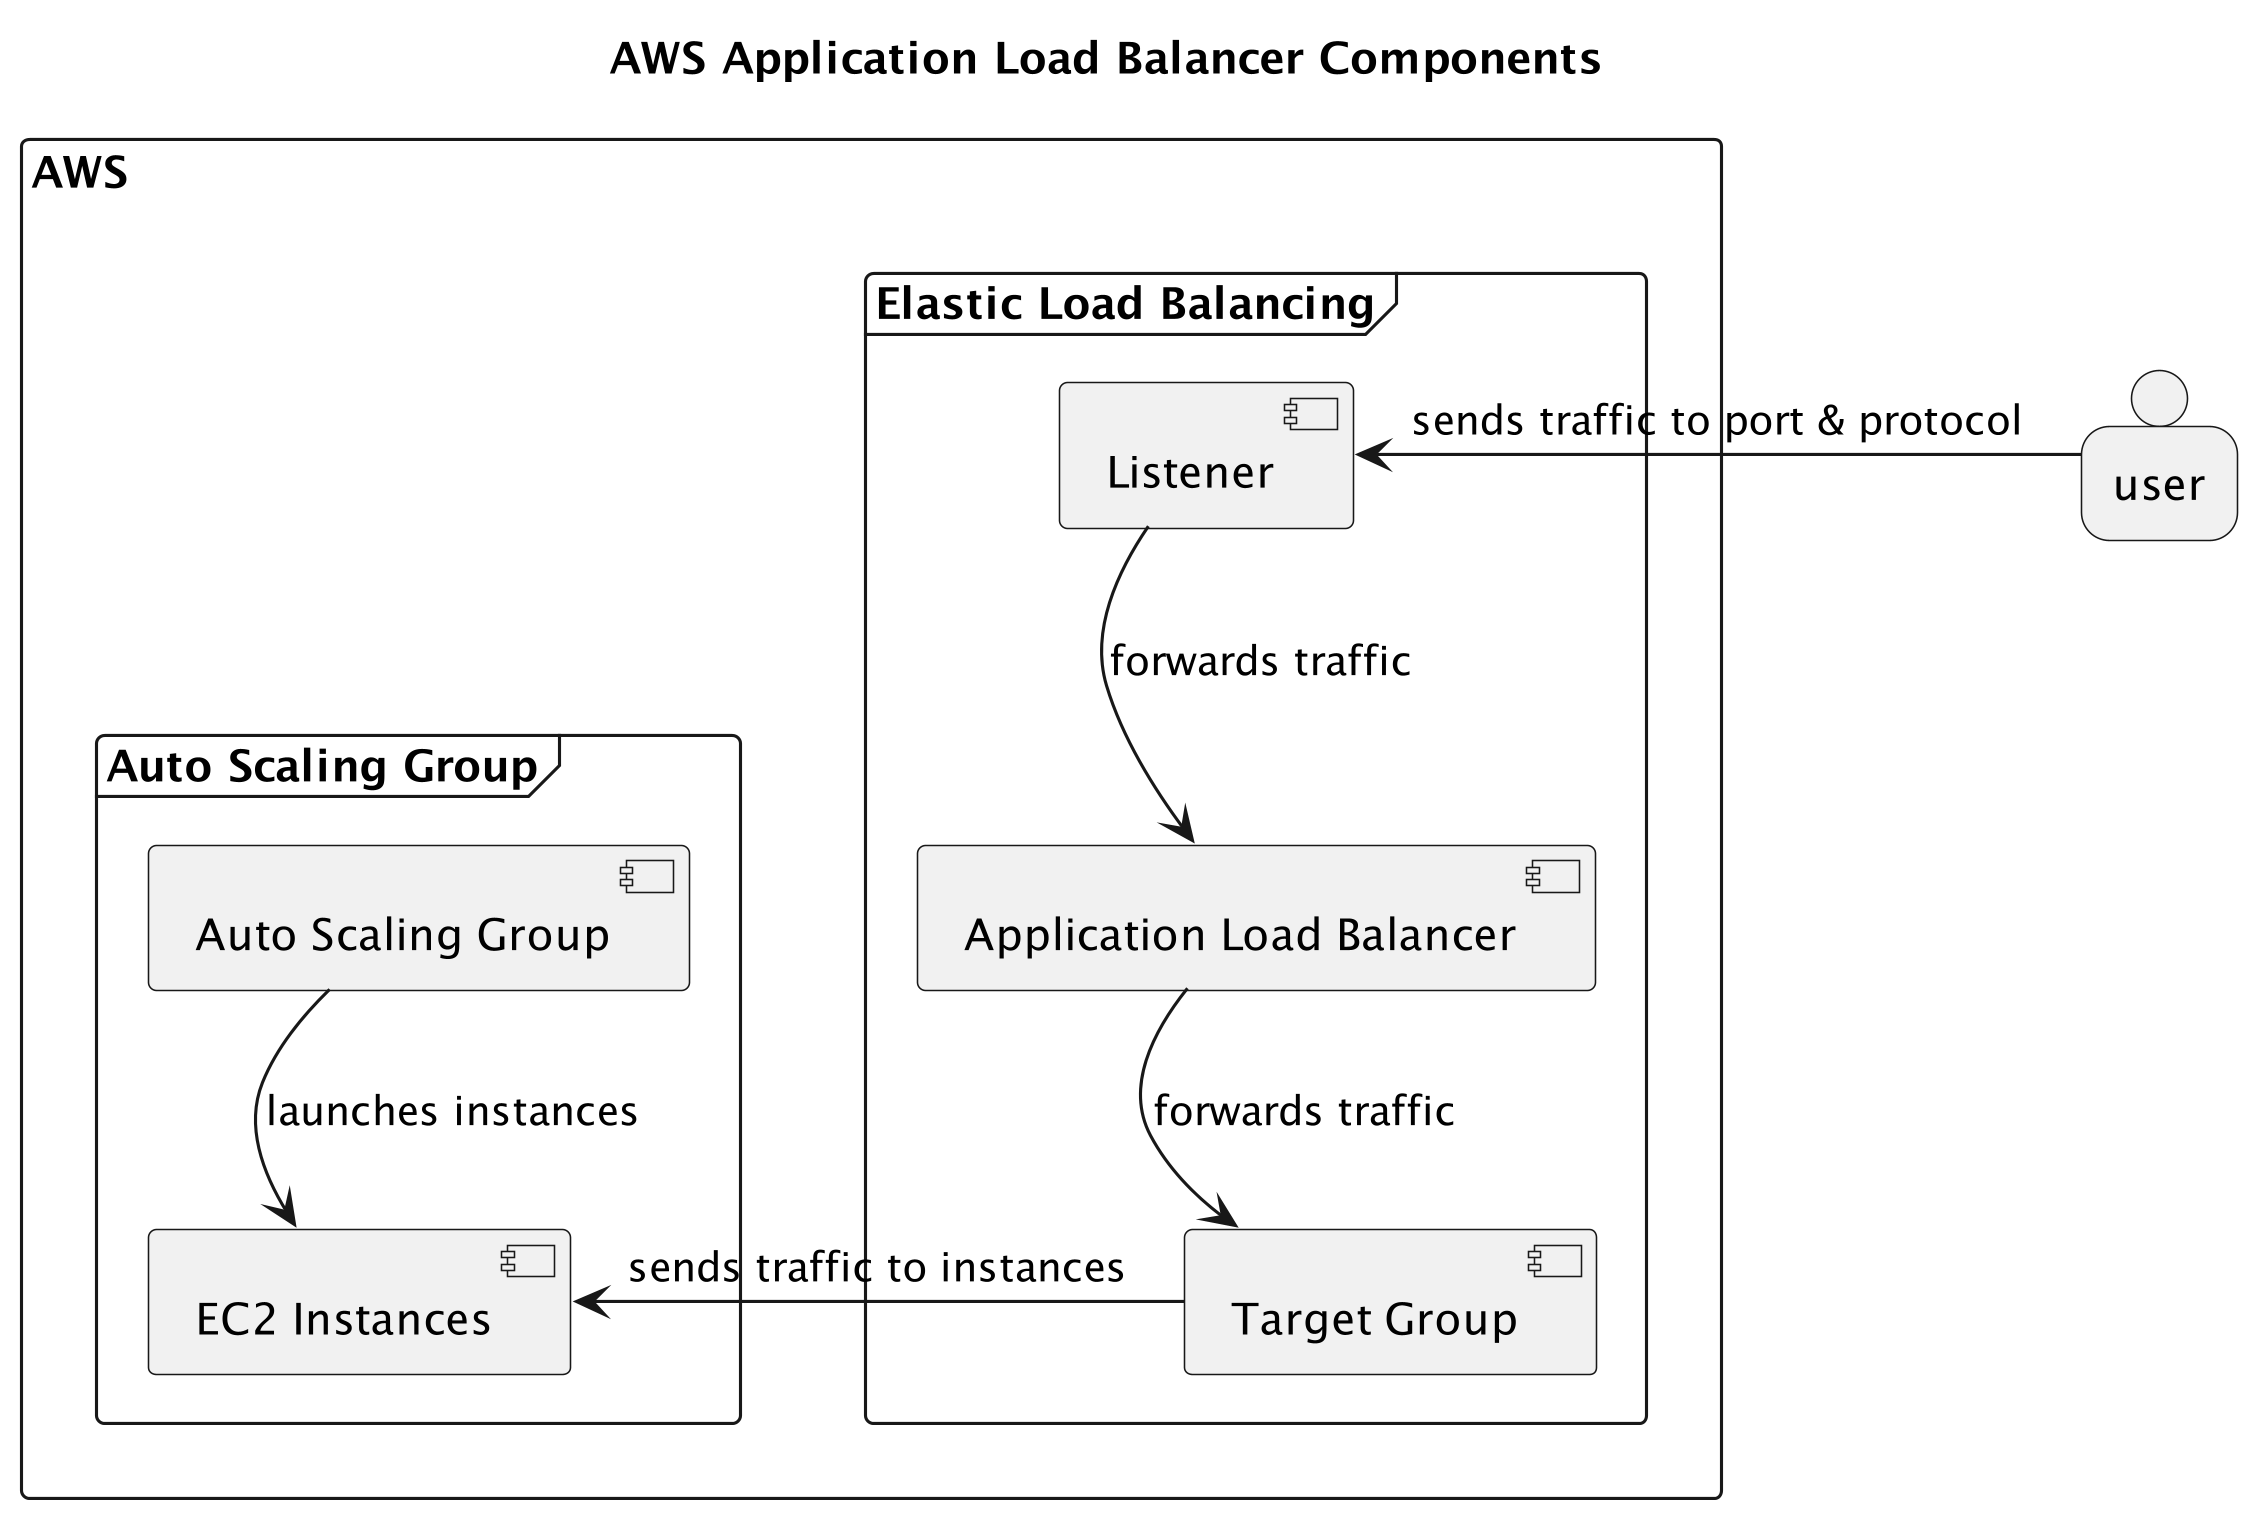
\includegraphics[width=\textwidth]{diagrams/loadbalancers}
\end{figure}

\subsection{Autoscaling in AWS}
Instead of creating the maxiumum amount of services we predict we will need,
we can automatically scale the number of nodes we need to minimise resources.
When the load is low, we operate with minimal nodes.
When the load is high, we increase the number of nodes available to cope.

To compute the resources needed, AWS relies on triggers from CloudWatch and scaling policies.
Some premade triggers are based around a node's;

\begin{itemize}
    \item CPU usage,
    \item memory usage, or 
    \item network usage.
\end{itemize}

We create custom triggers based on our application's metrics.

\section{Load Balancing TaskOverflow}

\subsection{[Path A] EC2}

\begin{figure}[H]
  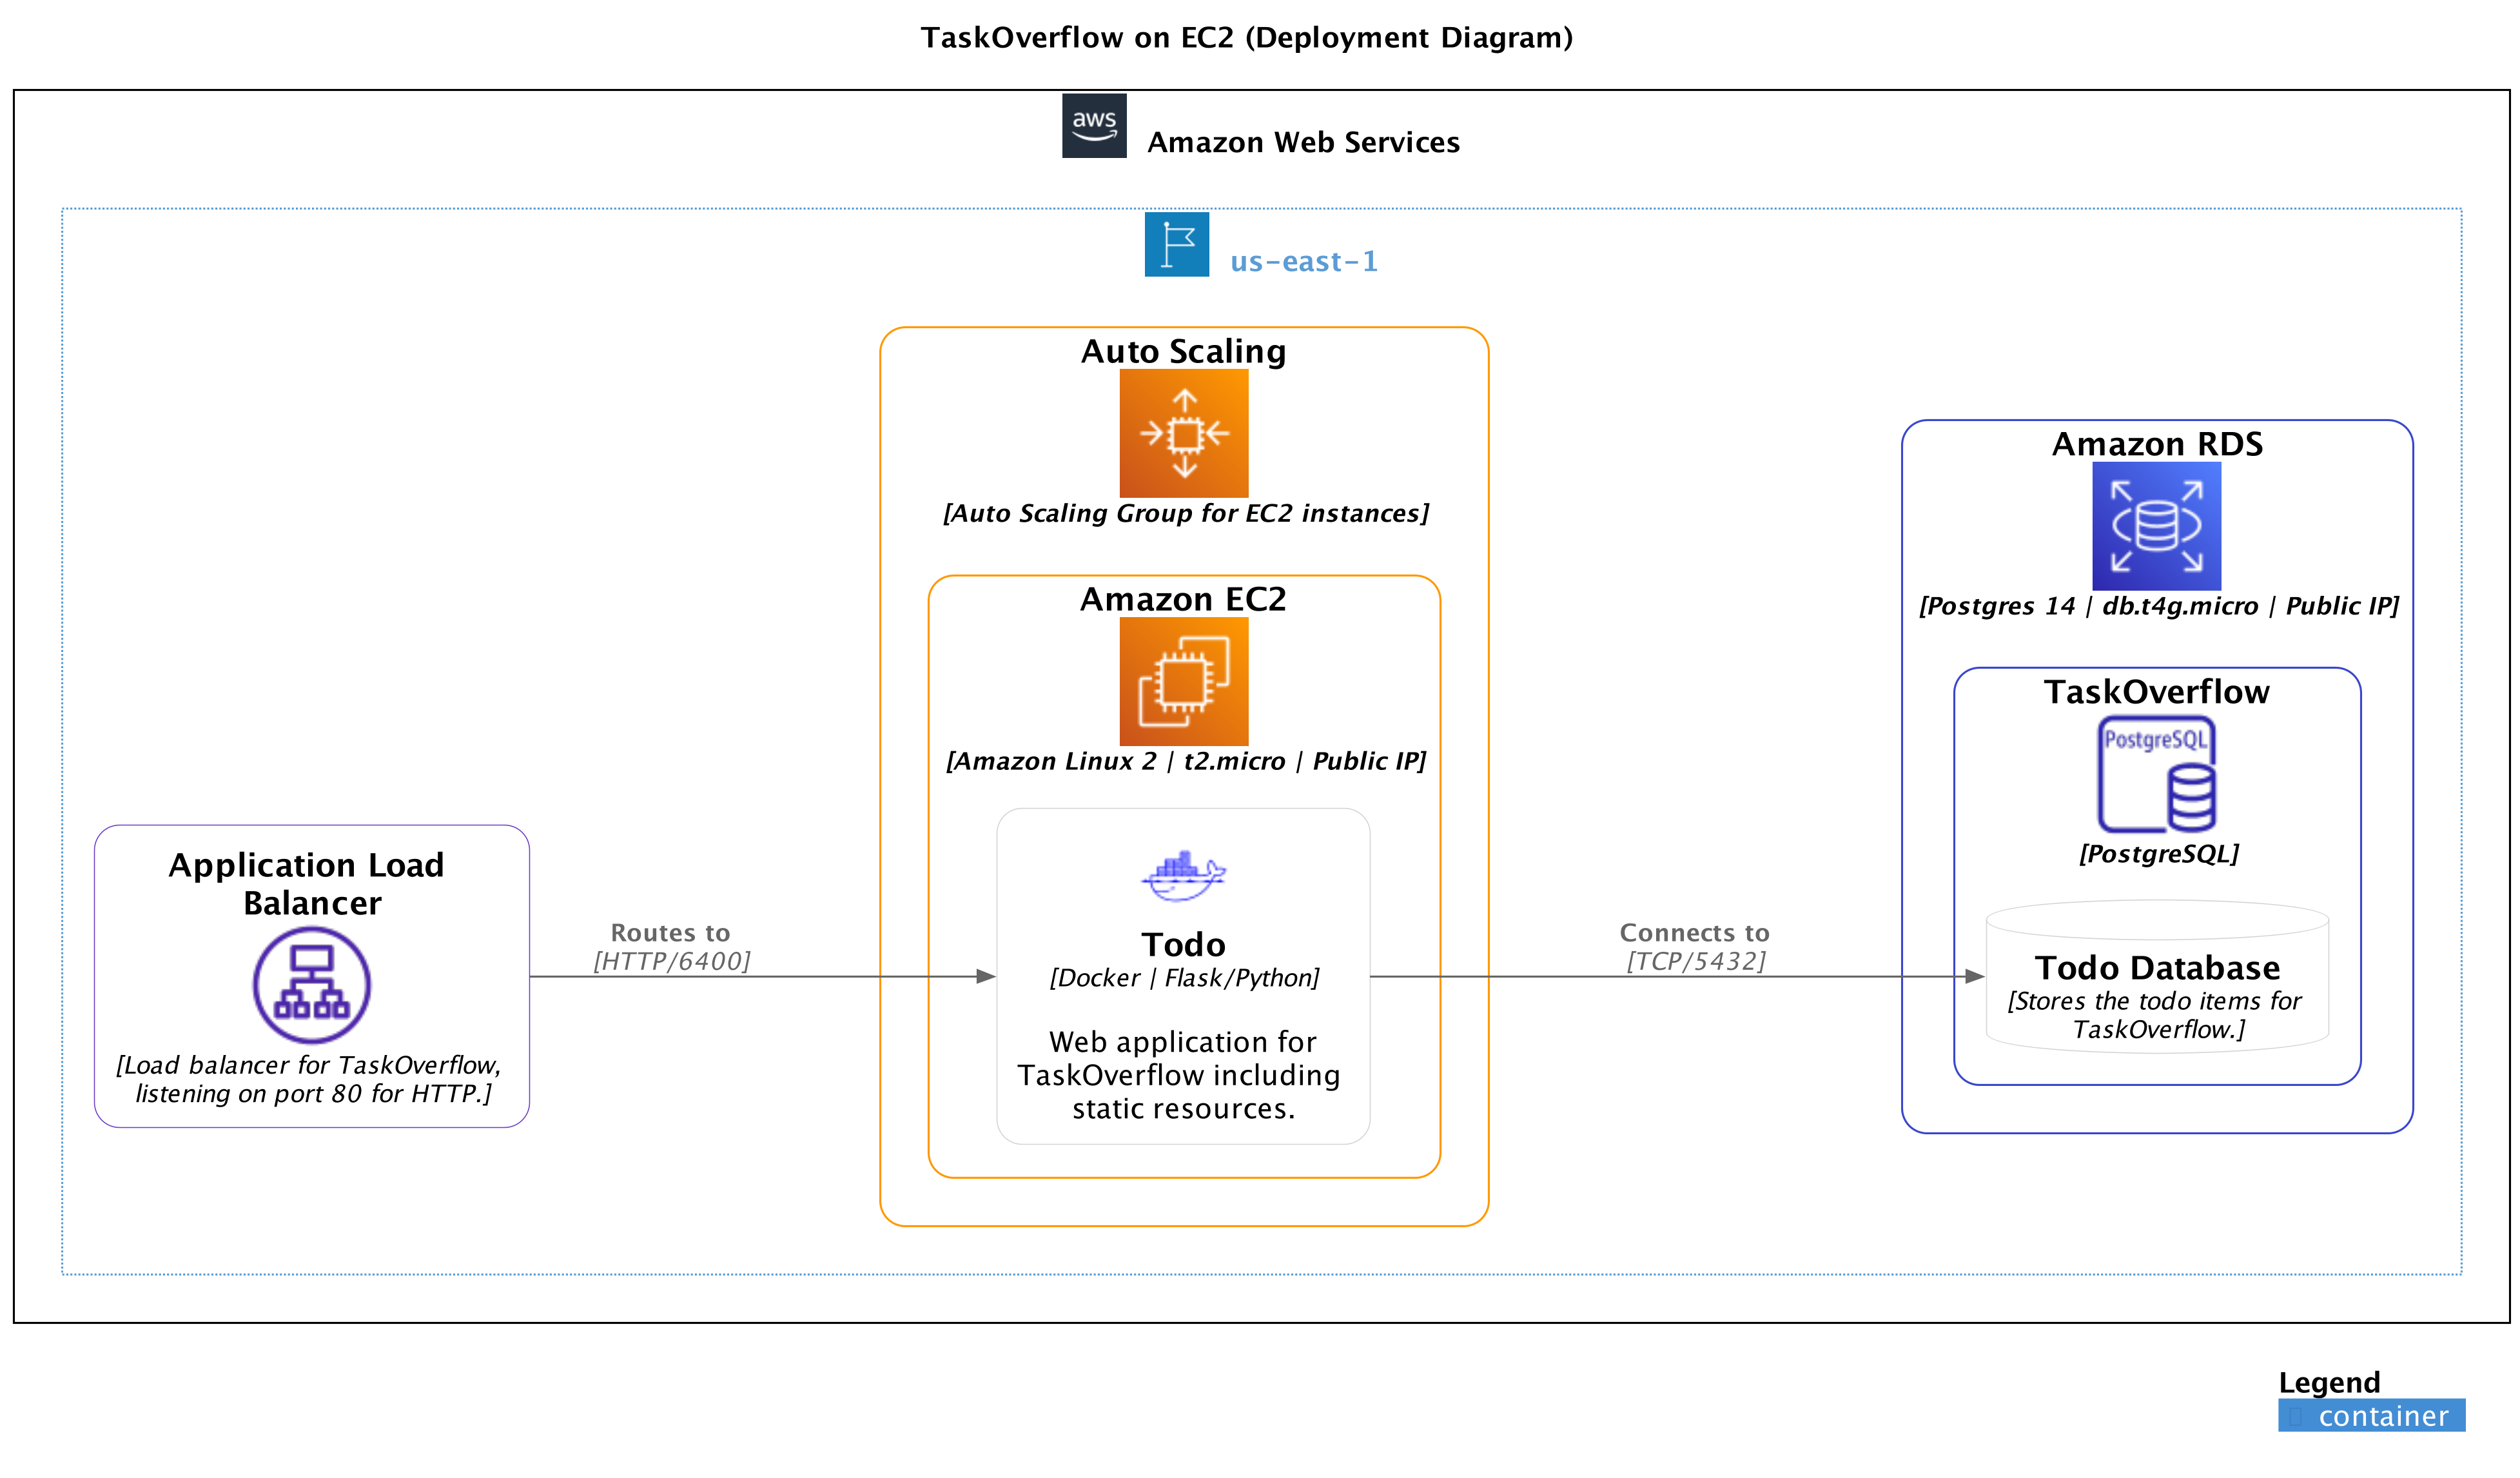
\includegraphics[width=\textwidth]{diagrams/ec2deployment}
\end{figure}

\todo{Move to EC2Template}



\begin{code}[language=terraform,numbers=none]{ec2.tf}
resource "aws_launch_template" "todo" {
  name = "todo-launch-template"
  image_id = "ami-005f9685cb30f234b"
  instance_type = "t2.micro"
  key_name = "vockey"

  user_data = base64encode(<<-EOT
    #!/bin/bash
    yum update -y
    yum install -y docker
    service docker start
    systemctl enable docker
    usermod -a -G docker ec2-user 
    docker run --restart always -e SQLALCHEMY_DATABASE_URI=postgresql://${local.database_username}:${local.database_password}@${aws_db_instance.database.address}:5432/todo -p 6400:6400 ${local.image}
EOT
  )

  vpc_security_group_ids = [aws_security_group.todo.id]
}


resource "aws_security_group" "todo" {
  name = "todo"
  description = "TaskOverflow Security Group"

  ingress {
    from_port = 6400
    to_port = 6400
    protocol = "tcp"
    cidr_blocks = ["0.0.0.0/0"]
  }

  ingress {
    from_port = 22
    to_port = 22
    protocol = "tcp"
    cidr_blocks = ["0.0.0.0/0"]
  }

  egress {
    from_port = 0
    to_port = 0
    protocol = "-1"
    cidr_blocks = ["0.0.0.0/0"]
  }
}
\end{code}

\todo{AutoScaling group}

\begin{figure}[H]
  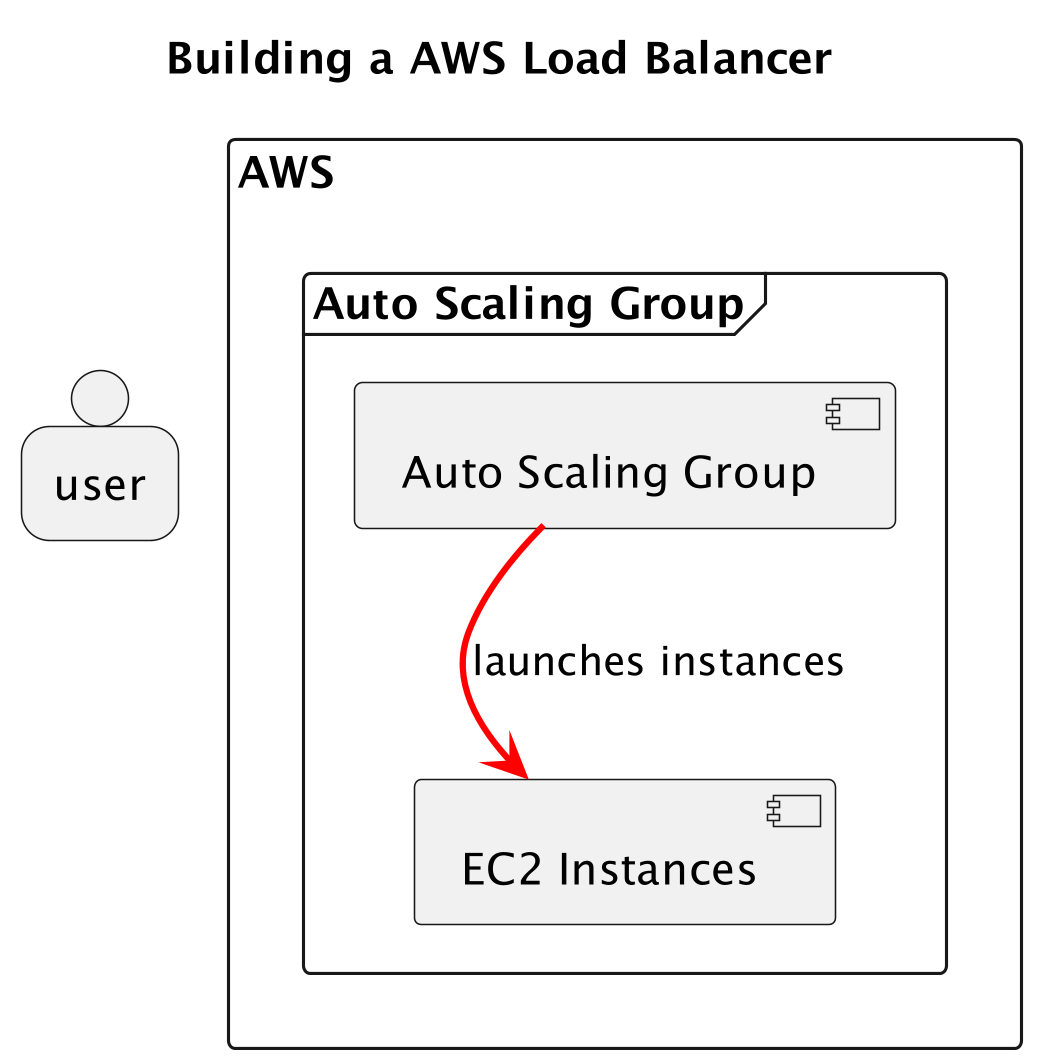
\includegraphics[width=\textwidth]{diagrams/lb1}
\end{figure}

\begin{code}[language=terraform,numbers=none]{autoscaling.tf}
resource "aws_autoscaling_group" "todo" {
  name = "todo"
  availability_zones = ["us-east-1a"]
  desired_capacity   = 1
  max_size           = 4
  min_size           = 1
  
  launch_template {
    id      = aws_launch_template.todo.id
    version = "$Latest"
  }
}
\end{code}

\todo{target group}

\begin{figure}[H]
  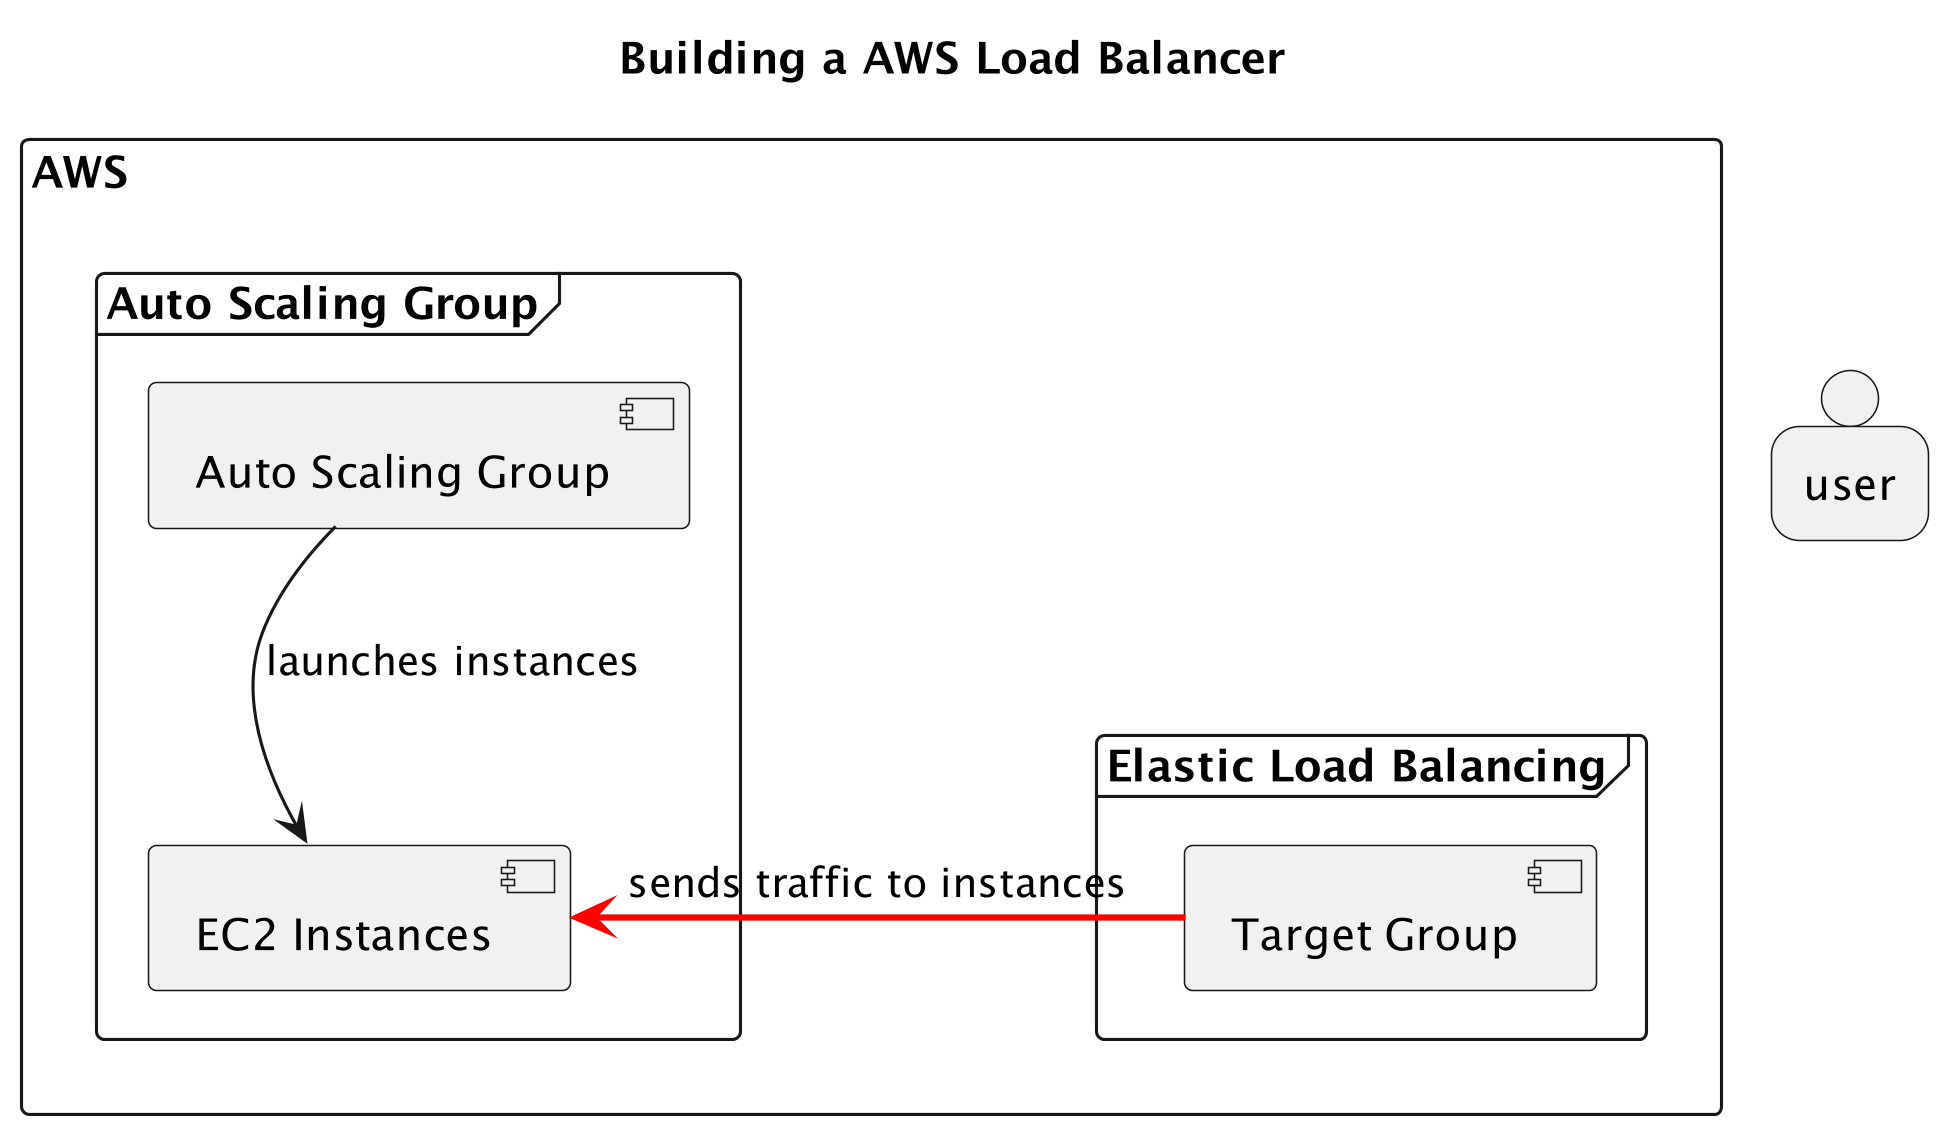
\includegraphics[width=\textwidth]{diagrams/lb2}
\end{figure}

\begin{code}[language=terraform,numbers=none]{lb.tf}
resource "aws_lb_target_group" "todo" {
  name     = "todo"
  port     = 6400
  protocol = "HTTP"
  vpc_id   = aws_security_group.todo.vpc_id
}
\end{code}

\todo{autoscaling + target}

\begin{code}[language=terraform,numbers=none]{lb.tf}
resource "aws_autoscaling_attachment" "todo" {
  autoscaling_group_name = aws_autoscaling_group.todo.id
  alb_target_group_arn   = aws_lb_target_group.todo.arn
}
\end{code}

\todo{load balancer}

\begin{figure}[H]
  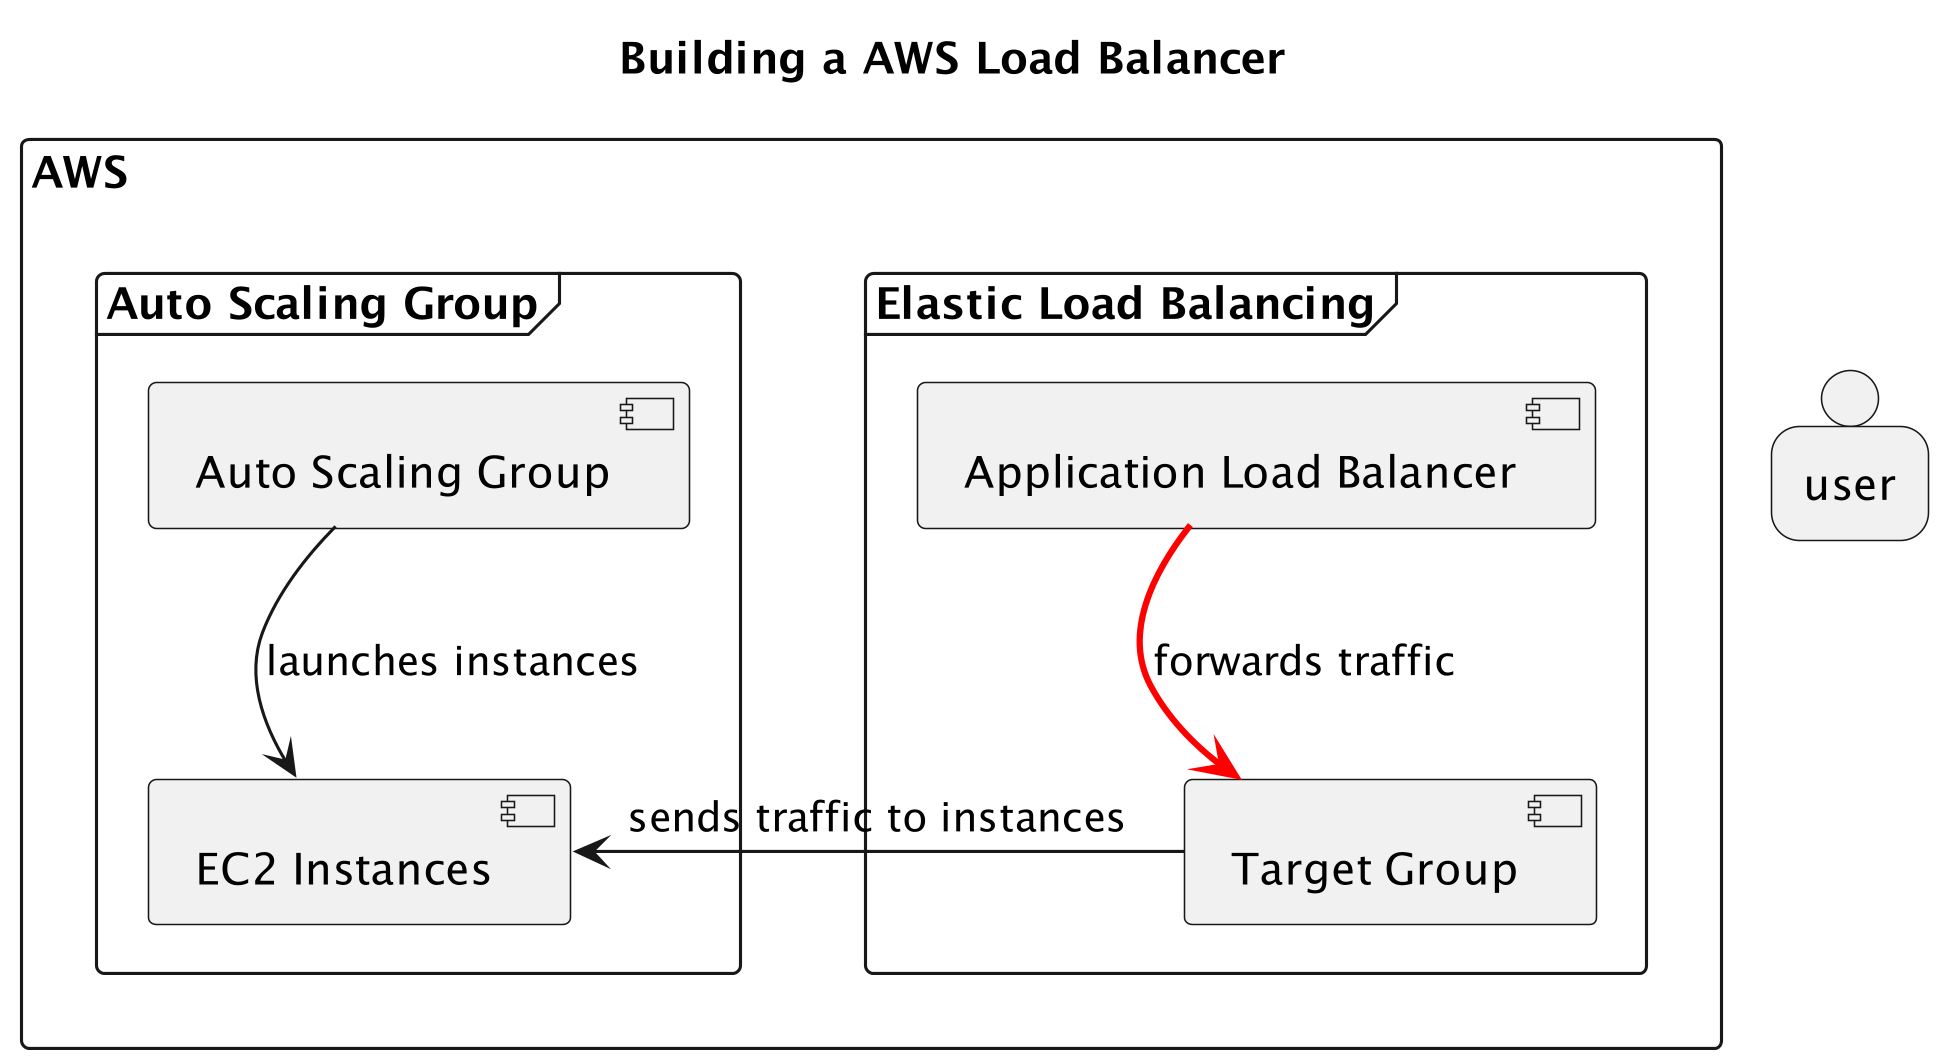
\includegraphics[width=\textwidth]{diagrams/lb3}
\end{figure}

\begin{code}[language=terraform,numbers=none]{lb.tf}
resource "aws_lb" "taskoverflow" {
  name               = "taskoverflow"
  internal           = false
  load_balancer_type = "application"
  subnets            = data.aws_subnets.private.ids
  security_groups    = [aws_security_group.taskoverflow.id]
}

resource "aws_security_group" "taskoverflow" {
  name = "taskoverflow"
  description = "TaskOverflow Security Group"

  ingress {
    from_port = 80
    to_port = 80
    protocol = "tcp"
    cidr_blocks = ["0.0.0.0/0"]
  }

  egress {
    from_port = 0
    to_port = 0
    protocol = "-1"
    cidr_blocks = ["0.0.0.0/0"]
  }
}
\end{code}

\todo{listener}

\begin{figure}[H]
  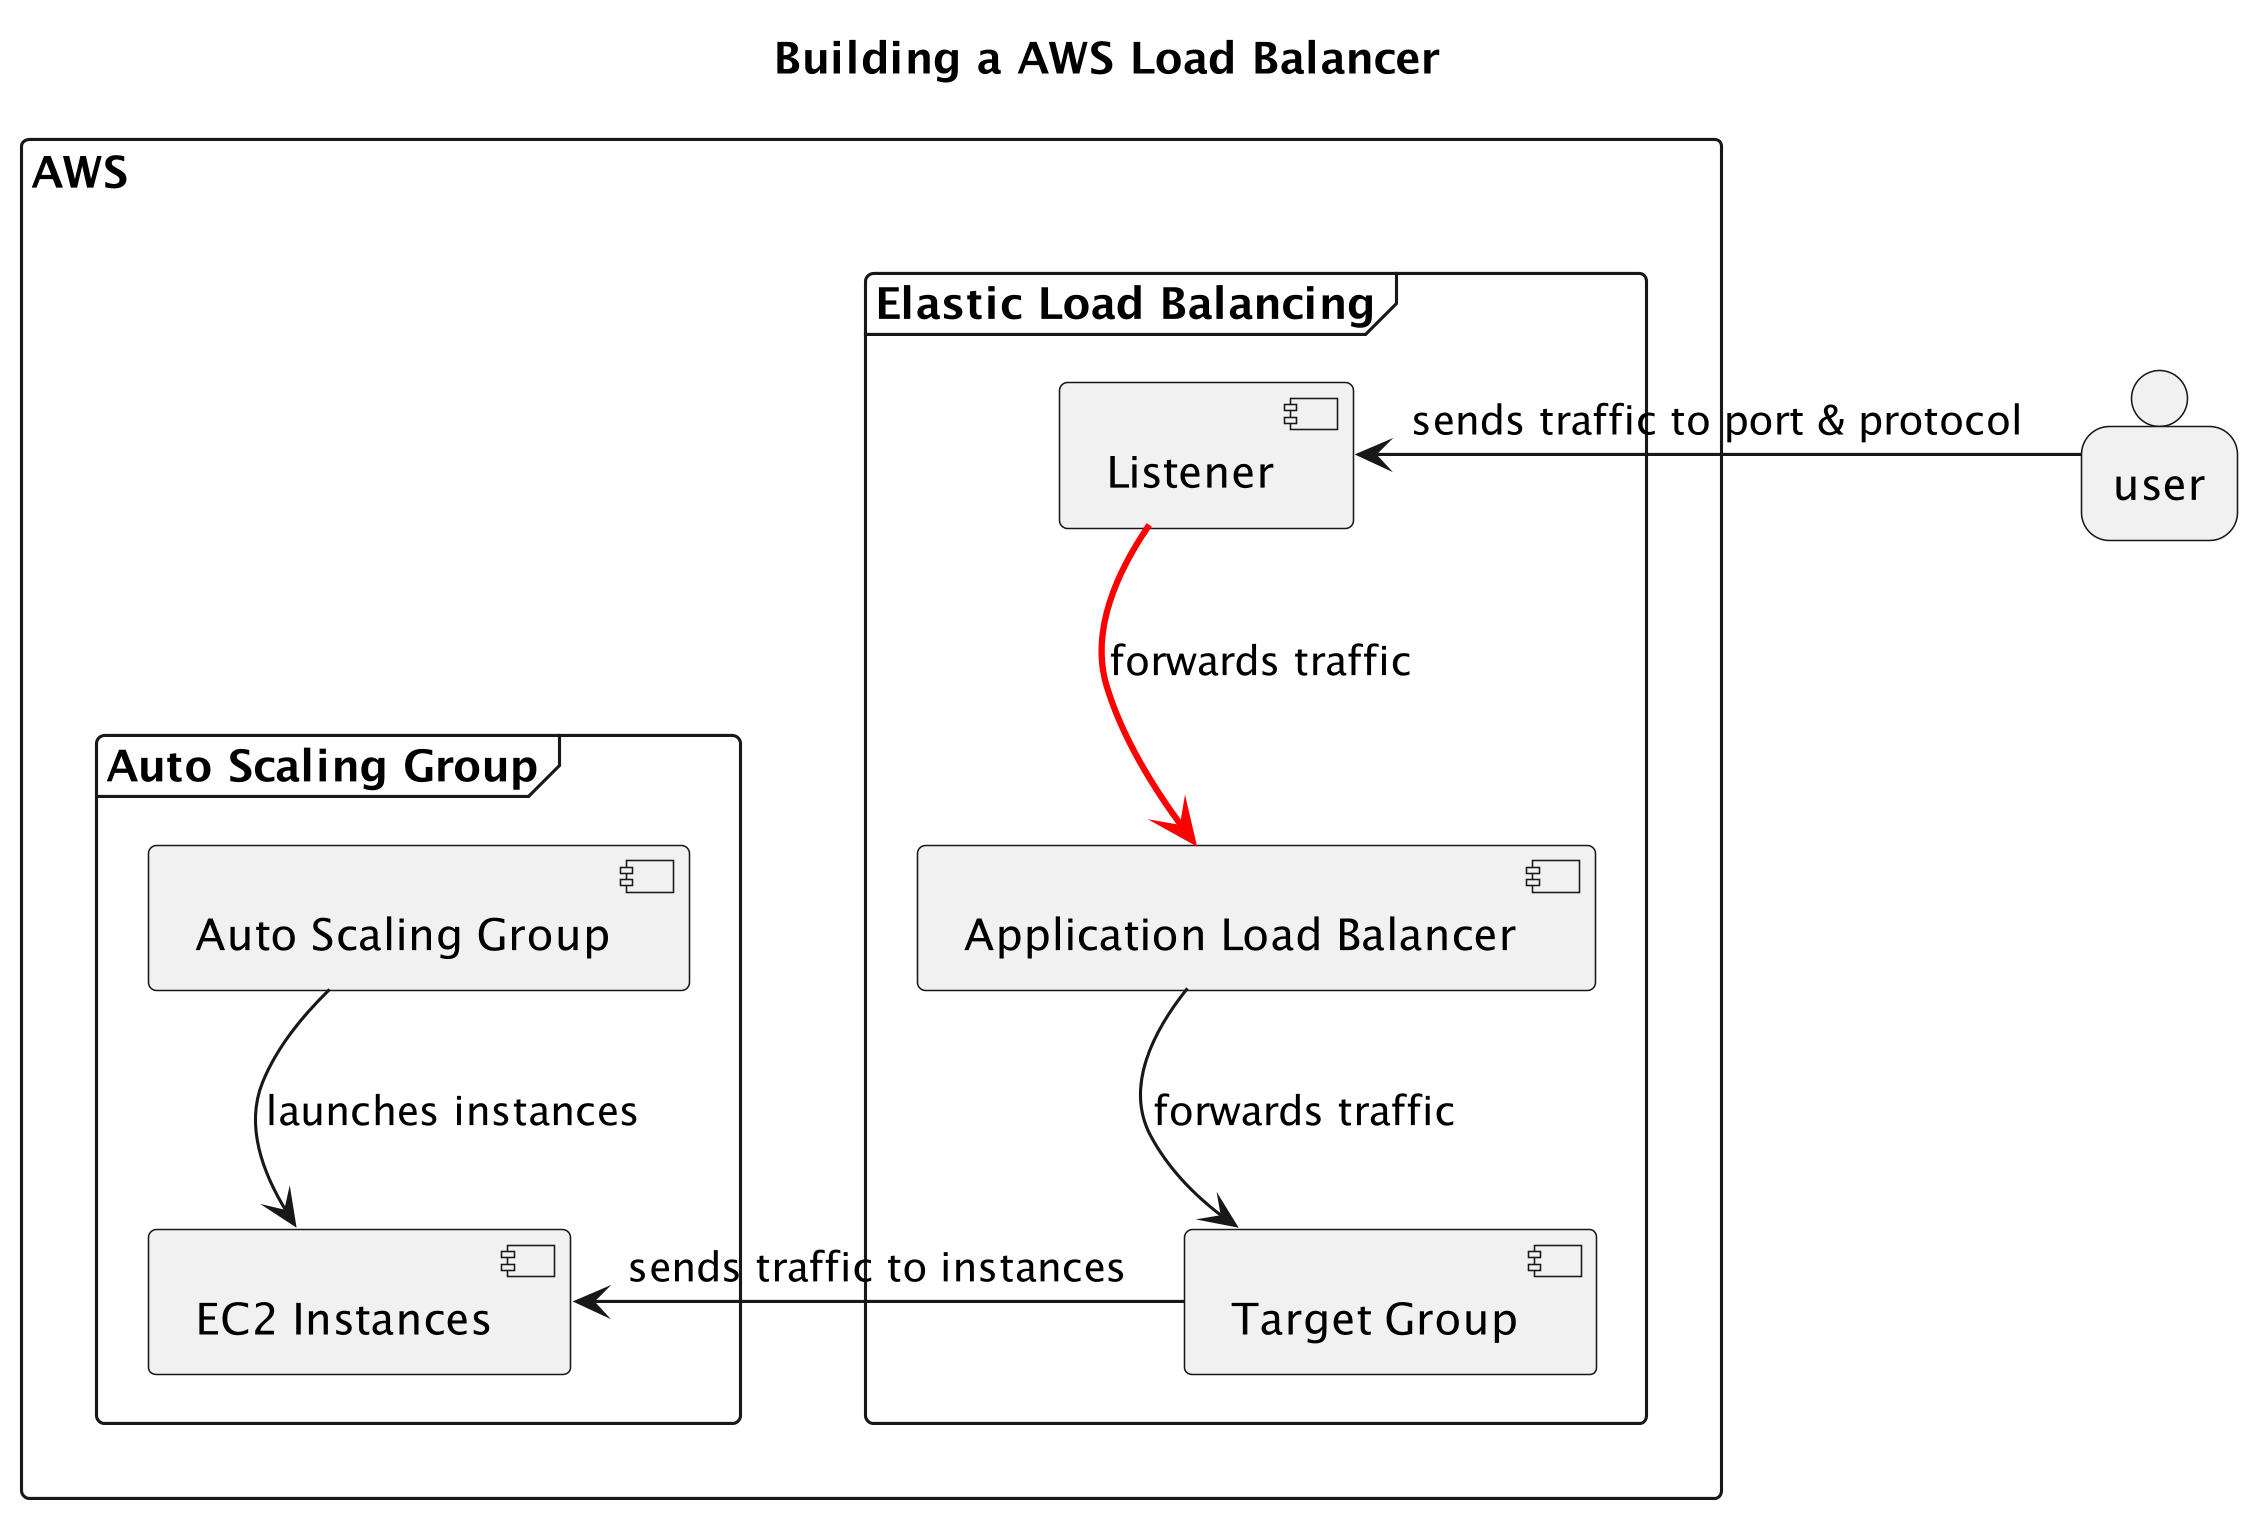
\includegraphics[width=\textwidth]{diagrams/lb4}
\end{figure}

\begin{code}[language=terraform,numbers=none]{lb.tf}
resource "aws_lb_listener" "taskoverflow" {
  load_balancer_arn = aws_lb.taskoverflow.arn
  port              = "80"
  protocol          = "HTTP"

  default_action {
    type             = "forward"
    target_group_arn = aws_lb_target_group.todo.arn
  }
}
\end{code}

\todo{Applying autoscaling rules}

\begin{code}[language=terraform,numbers=none]{autoscaling.tf}
resource "aws_autoscaling_policy" "todo_scale_down" {
  name                   = "todo_scale_down"
  autoscaling_group_name = aws_autoscaling_group.todo.name
  adjustment_type        = "ChangeInCapacity"
  scaling_adjustment     = -1
  cooldown               = 120
}

resource "aws_cloudwatch_metric_alarm" "todo_scale_down" {
  alarm_description   = "Monitors CPU utilization for Todo"
  alarm_actions       = [aws_autoscaling_policy.todo_scale_down.arn]
  alarm_name          = "todo_scale_down"
  comparison_operator = "LessThanOrEqualToThreshold"
  namespace           = "AWS/EC2"
  metric_name         = "CPUUtilization"
  threshold           = "10"
  evaluation_periods  = "2"
  period              = "120"
  statistic           = "Average"

  dimensions = {
    AutoScalingGroupName = aws_autoscaling_group.todo.name
  }
}

resource "aws_autoscaling_policy" "todo_scale_up" {
  name                   = "todo_scale_up"
  autoscaling_group_name = aws_autoscaling_group.todo.name
  adjustment_type        = "ChangeInCapacity"
  scaling_adjustment     = 1
  cooldown               = 120
}

resource "aws_cloudwatch_metric_alarm" "todo_scale_up" {
  alarm_description   = "Monitors CPU utilization for Todo"
  alarm_actions       = [aws_autoscaling_policy.todo_scale_up.arn]
  alarm_name          = "todo_scale_up"
  comparison_operator = "GreaterThanThreshold"
  namespace           = "AWS/EC2"
  metric_name         = "CPUUtilization"
  threshold           = "20"
  evaluation_periods  = "2"
  period              = "120"
  statistic           = "Average"

  dimensions = {
    AutoScalingGroupName = aws_autoscaling_group.todo.name
  }
}
\end{code}
\subsection{[Path B] ECS}

\begin{figure}[H]
  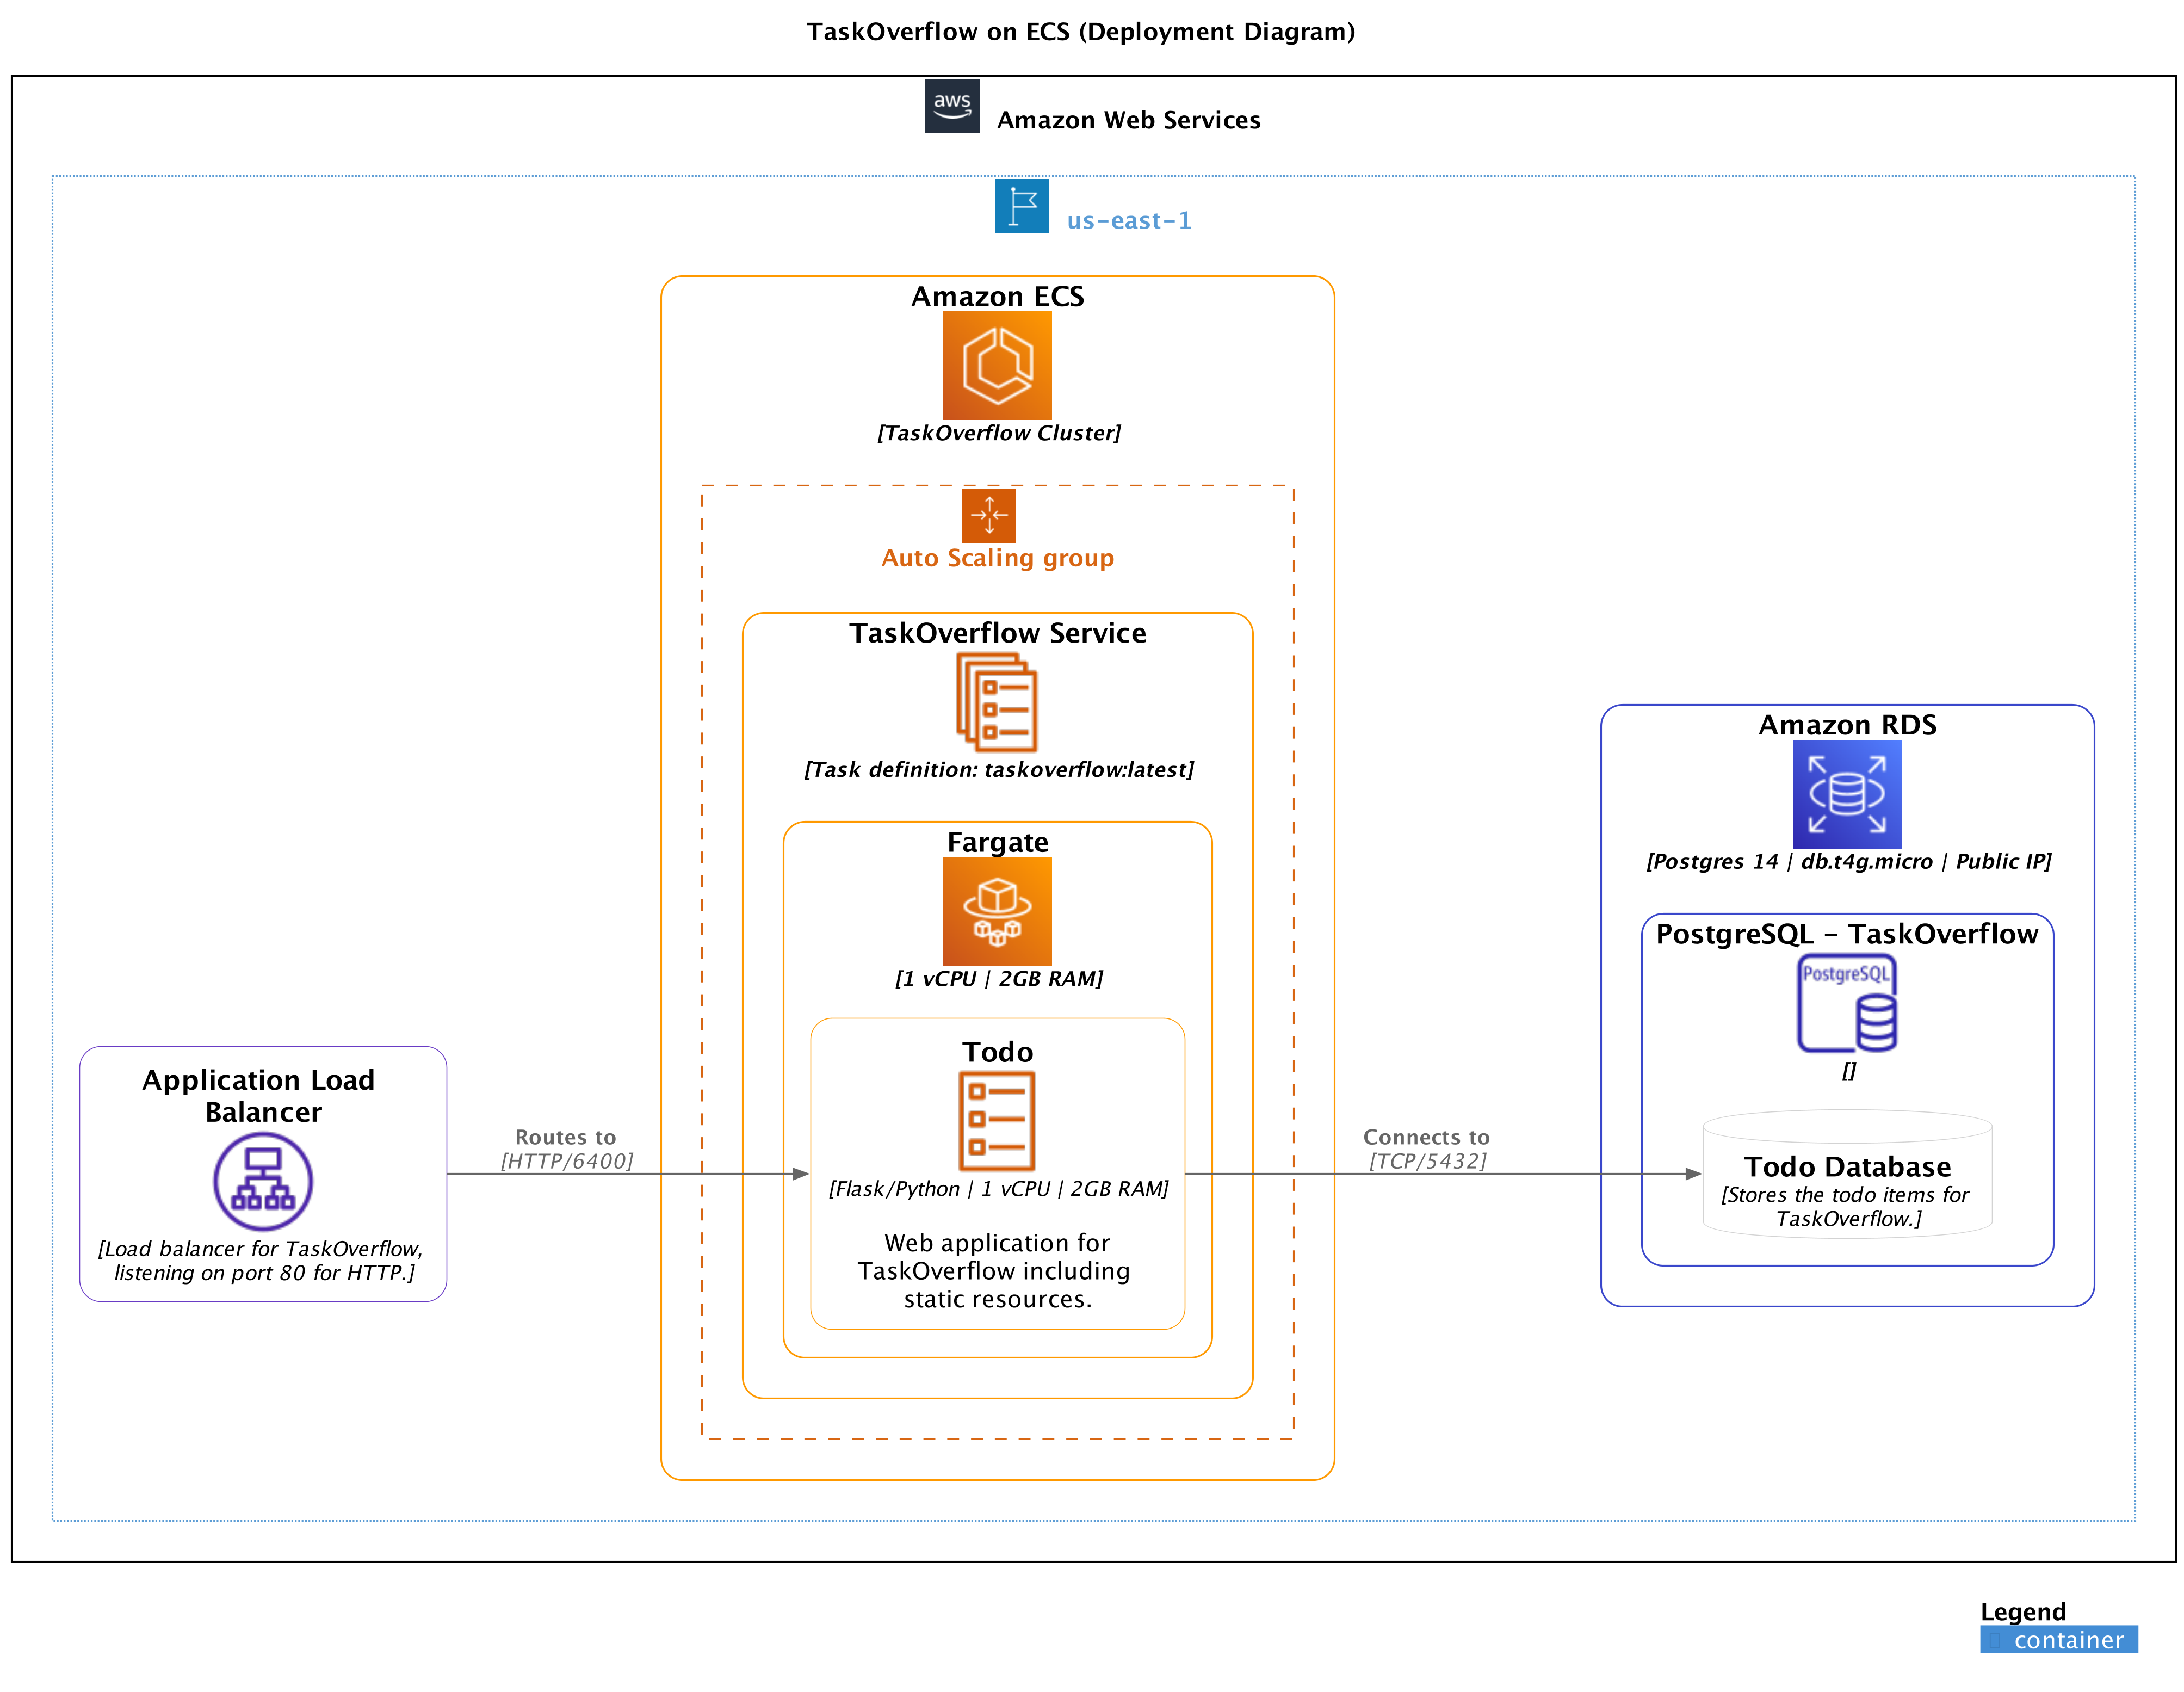
\includegraphics[width=\textwidth]{diagrams/ecsdeployment}
\end{figure}

\todo{target group}

\begin{figure}[H]
  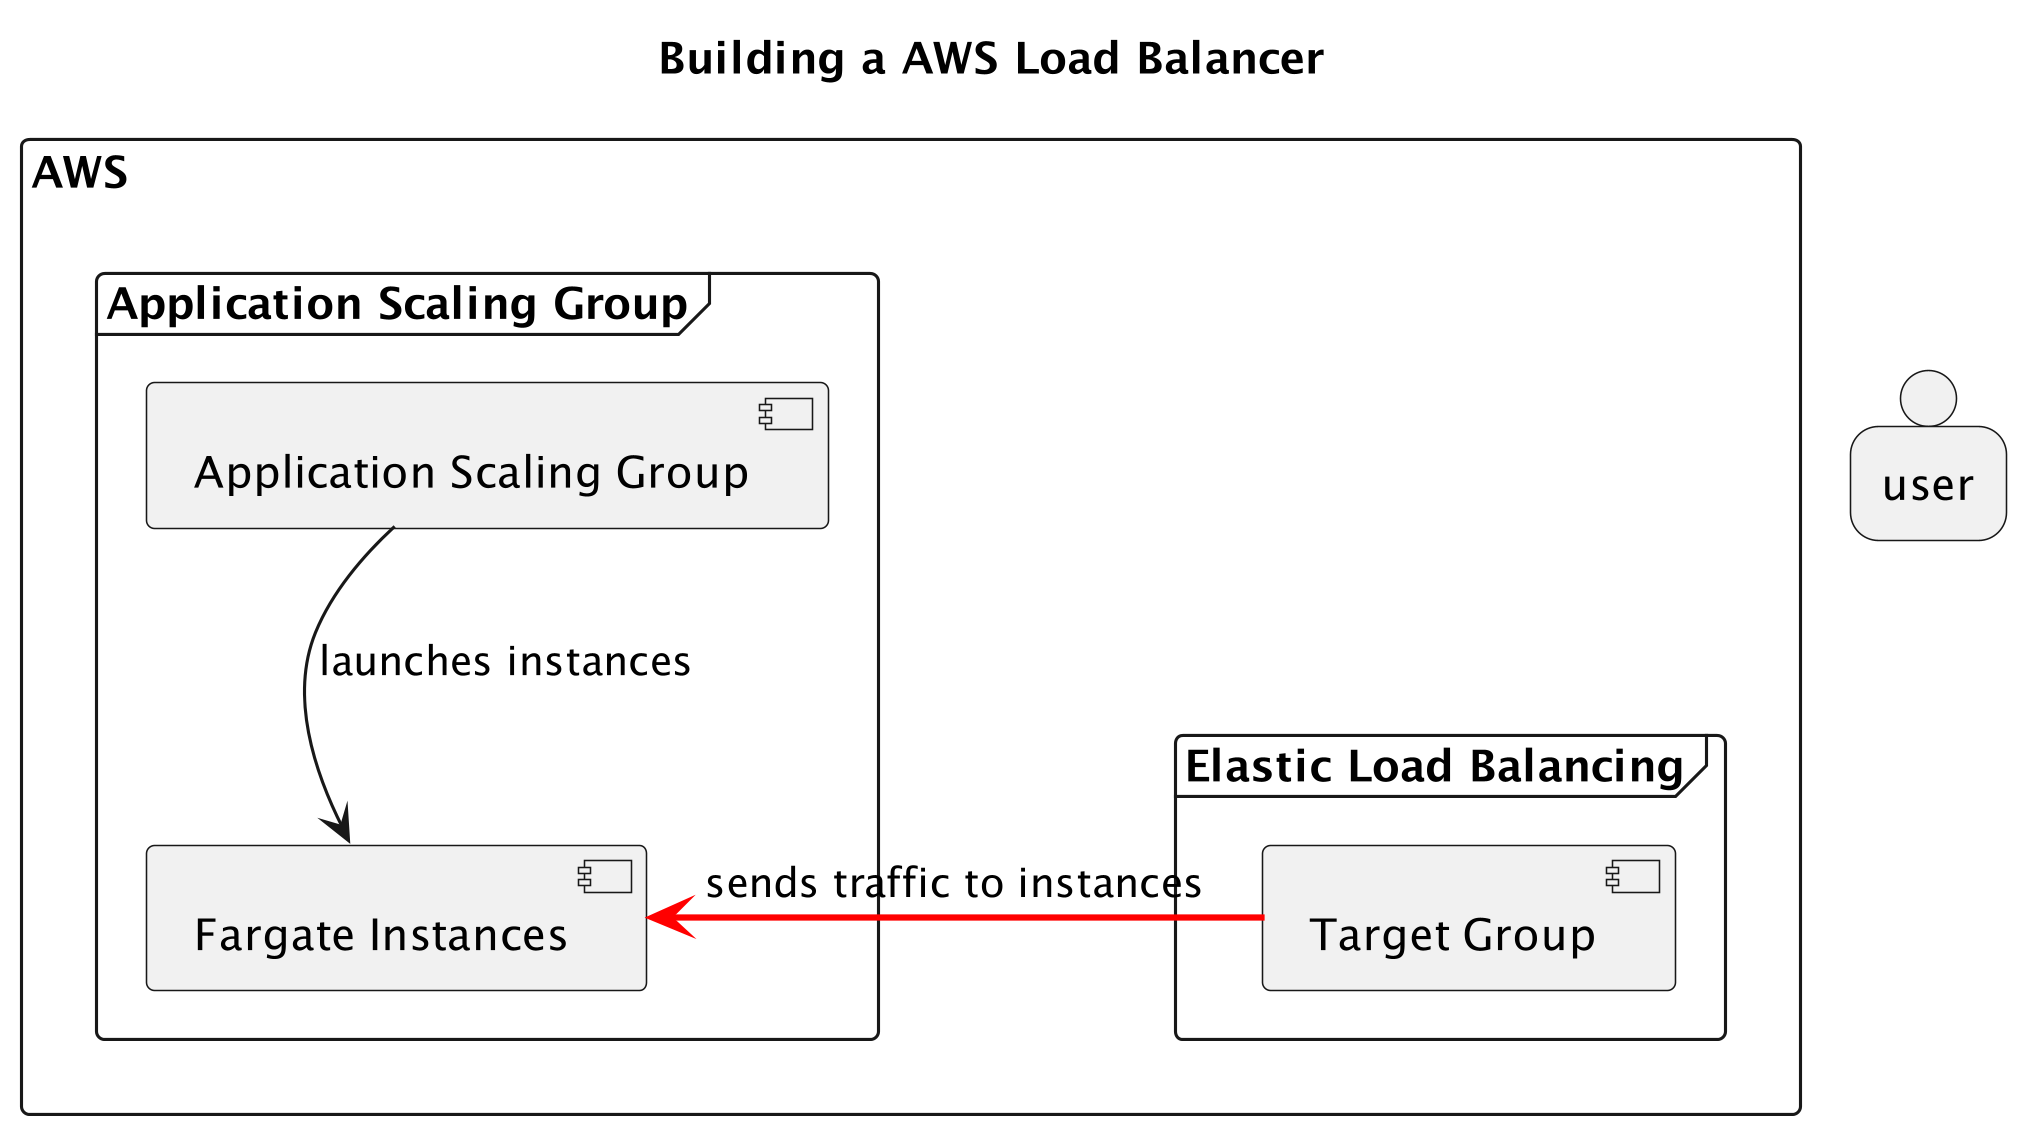
\includegraphics[width=\textwidth]{diagrams/lb2fargate.png}
\end{figure}

\begin{code}[language=terraform,numbers=none]{lb.tf}
resource "aws_lb_target_group" "todo" {
  name     = "todo"
  port     = 6400
  protocol = "HTTP"
  vpc_id   = aws_security_group.todo.vpc_id
  target_type = "ip"

  health_check {
    path = "/api/v1/health"
    port = "6400"
    protocol = "HTTP"
    healthy_threshold = 2
    unhealthy_threshold = 2
    timeout = 5
    interval = 10
  }
}
\end{code}

\todo{adding to ecs}

\begin{code}[language=terraform,numbers=none]{ecs.tf}
  load_balancer {
    target_group_arn = aws_lb_target_group.todo.arn
    container_name   = "todo"
    container_port   = 6400
  }
\end{code}

\todo{load balancer}

\begin{figure}[H]
  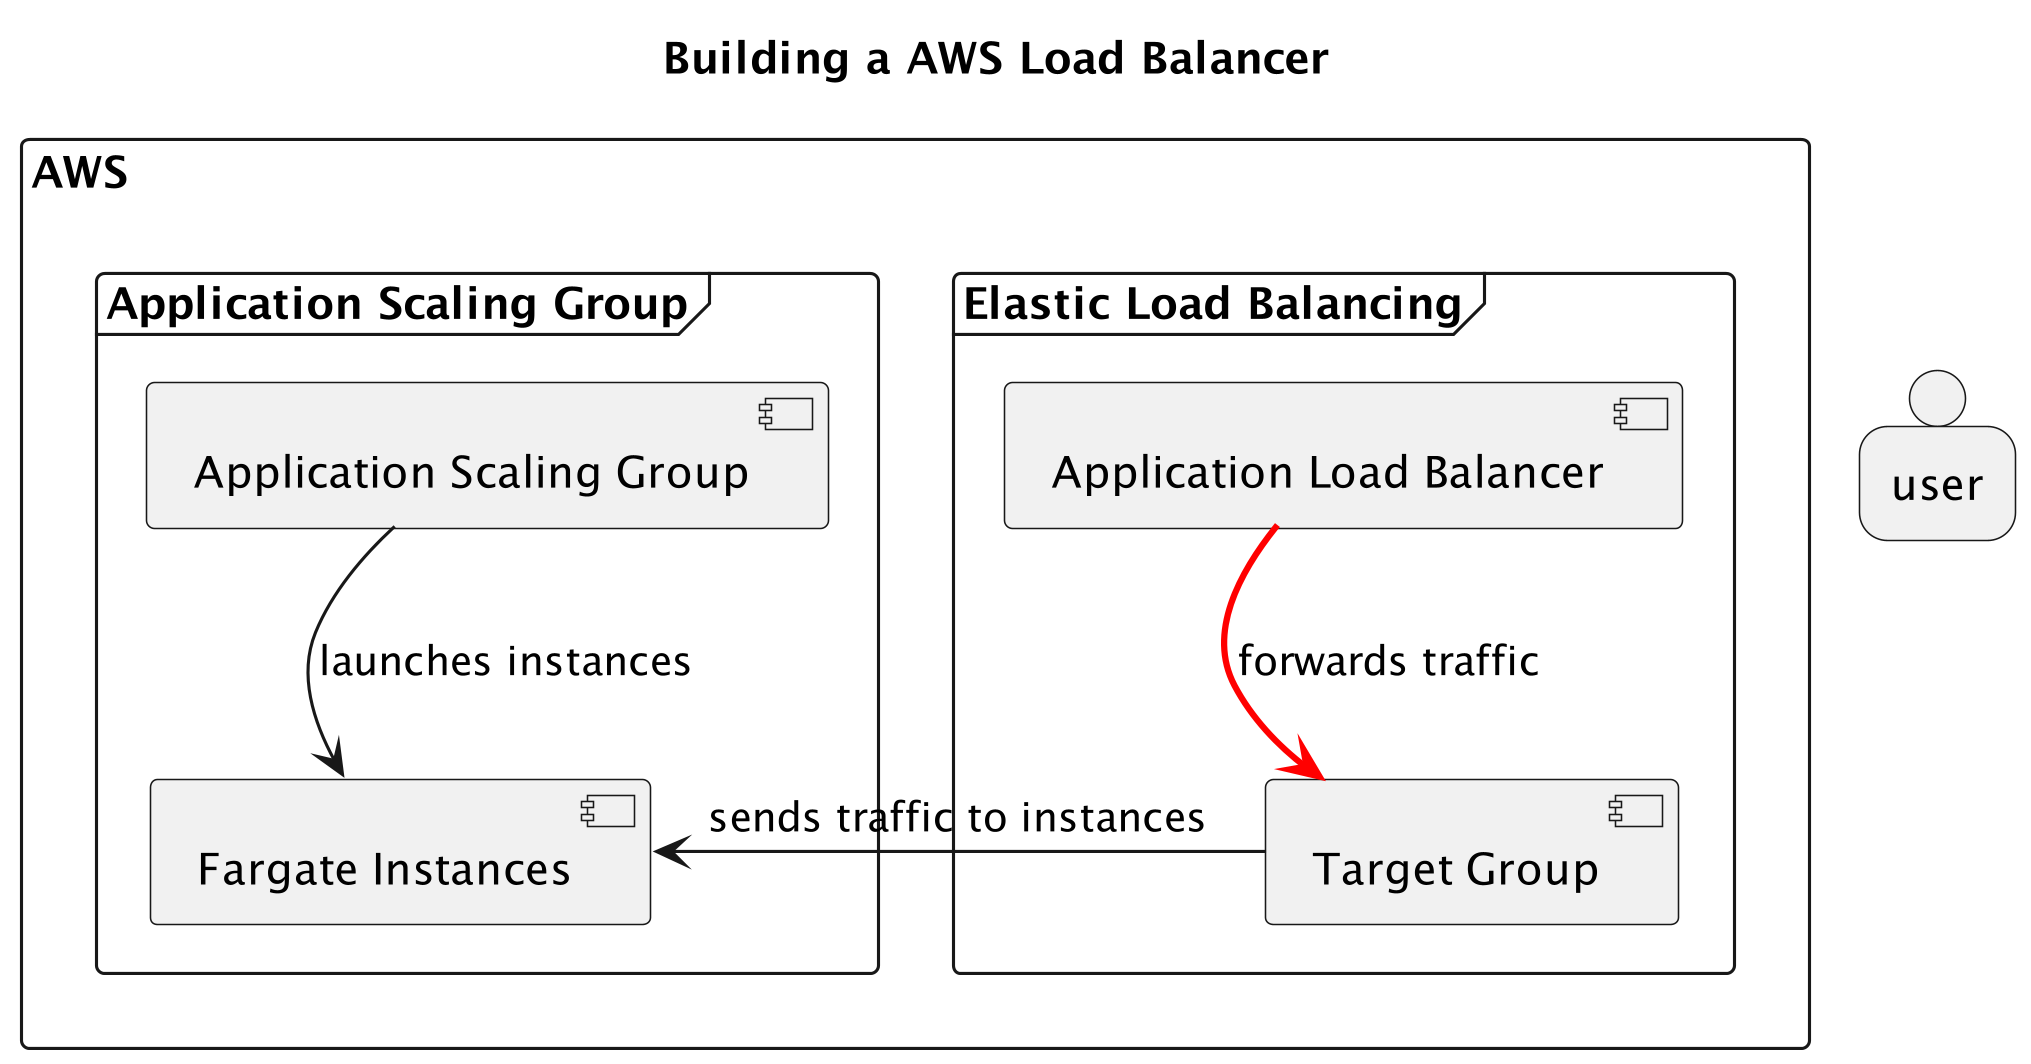
\includegraphics[width=\textwidth]{diagrams/lb3fargate}
\end{figure}

\begin{code}[language=terraform,numbers=none]{lb.tf}
resource "aws_lb" "taskoverflow" {
  name               = "taskoverflow"
  internal           = false
  load_balancer_type = "application"
  subnets            = data.aws_subnets.private.ids
  security_groups    = [aws_security_group.taskoverflow.id]
}

resource "aws_security_group" "taskoverflow" {
  name = "taskoverflow"
  description = "TaskOverflow Security Group"

  ingress {
    from_port = 80
    to_port = 80
    protocol = "tcp"
    cidr_blocks = ["0.0.0.0/0"]
  }

  egress {
    from_port = 0
    to_port = 0
    protocol = "-1"
    cidr_blocks = ["0.0.0.0/0"]
  }
}
\end{code}

\todo{listener}

\begin{figure}[H]
  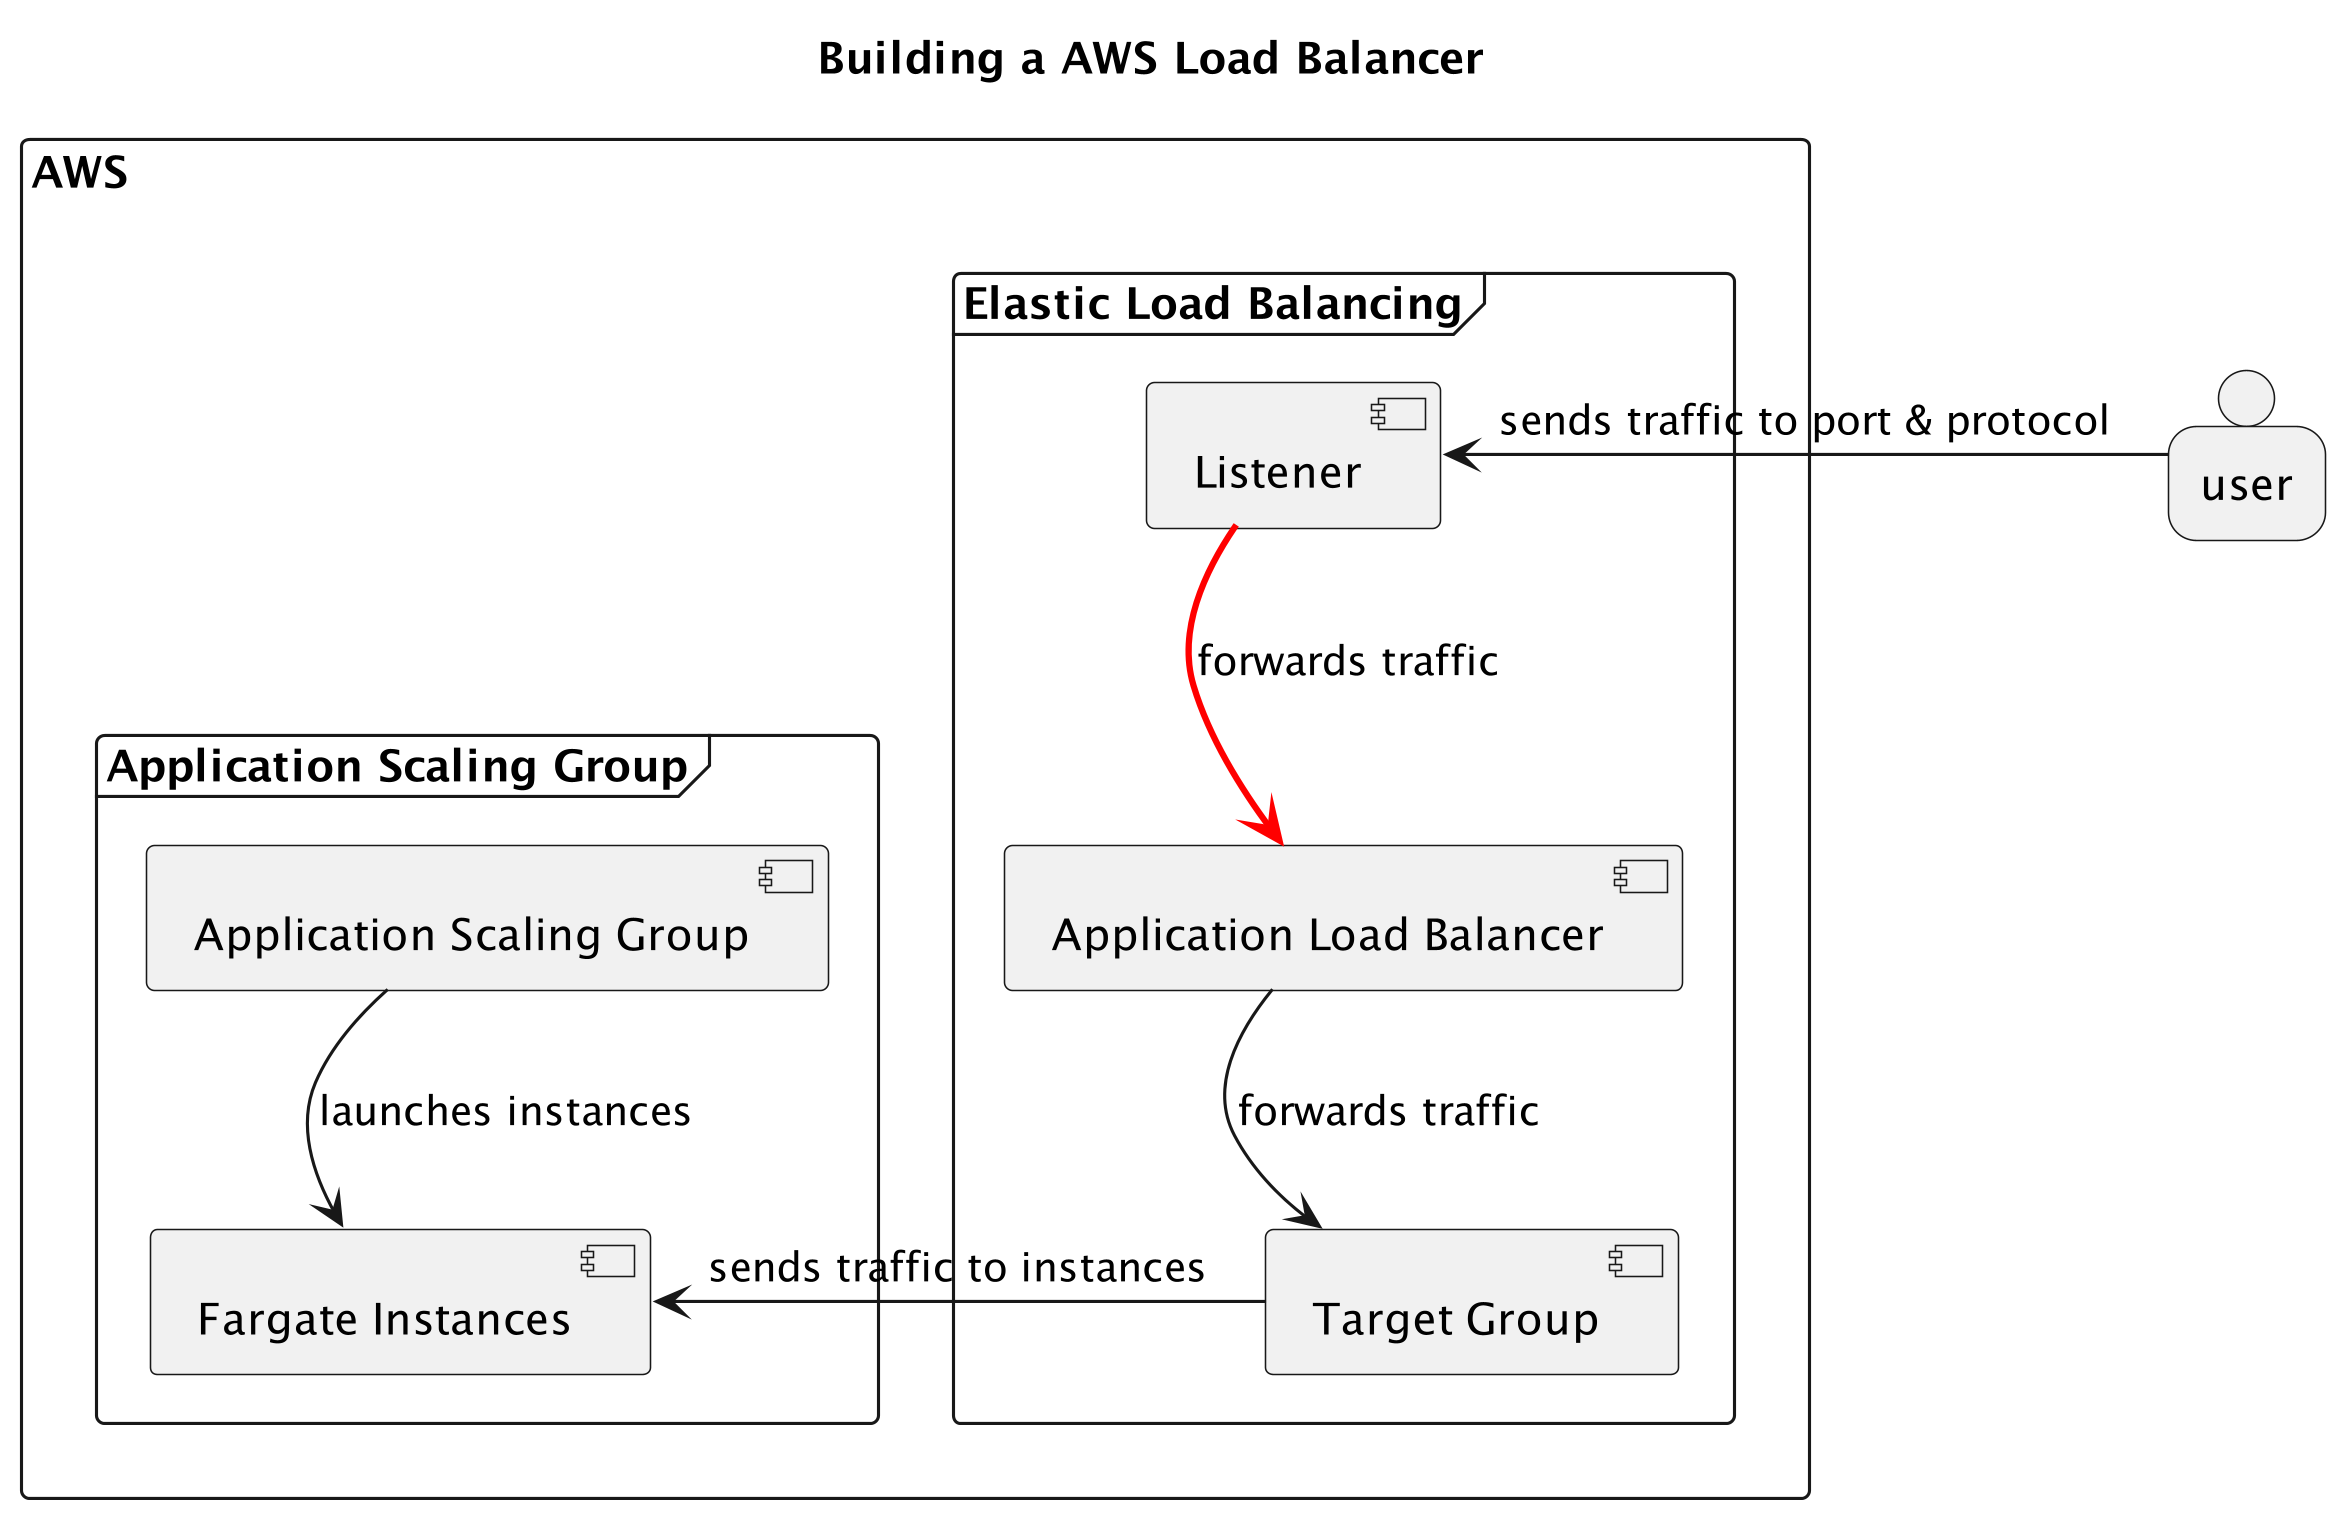
\includegraphics[width=\textwidth]{diagrams/lb4fargate}
\end{figure}

\begin{code}[language=terraform,numbers=none]{lb.tf}
resource "aws_lb_listener" "todo" {
  load_balancer_arn = aws_lb.taskoverflow.arn
  port              = "80"
  protocol          = "HTTP"

  default_action {
    type             = "forward"
    target_group_arn = aws_lb_target_group.todo.arn
  }
}
\end{code}

\todo{Applying autoscaling rules}

\begin{code}[language=terraform,numbers=none]{autoscaling.tf}
resource "aws_appautoscaling_target" "todo" {
  max_capacity = 4
  min_capacity = 1
  resource_id = "service/taskoverflow/taskoverflow"
  scalable_dimension = "ecs:service:DesiredCount"
  service_namespace = "ecs"
}


resource "aws_appautoscaling_policy" "todo-cpu" {
  name = "todo-cpu"
  policy_type = "TargetTrackingScaling"
  resource_id = aws_appautoscaling_target.todo.resource_id
  scalable_dimension = aws_appautoscaling_target.todo.scalable_dimension
  service_namespace = aws_appautoscaling_target.todo.service_namespace

  target_tracking_scaling_policy_configuration {
    predefined_metric_specification {
      predefined_metric_type = "ECSServiceAverageCPUUtilization"
    }

    target_value = 20
  }
}
\end{code}

\subsection{Producing Load with K6}

\begin{code}[language=javascript,numbers=none,escapechar=!]{k6.js}
import http from 'k6/http';
import { sleep, check } from 'k6';

export const options = {
  stages: [
    { target: 1000, duration: '1m' },
    { target: 5000, duration: '10m' },
  ],
};

export default function () {
  const res = http.get('http://!\colorbox{yellow}{<<Your LoadBalancer URL Here>>}!/api/v1/todos');
  check(res, { 'status was 200': (r) => r.status == 200 });
  sleep(1);
}
\end{code}


\bibliographystyle{ieeetr}
\bibliography{books,ours}

\end{document}
